% vim: ts=4 sts=4 sw=4 et tw=75
\chapter{定制 Vim}
\label{chap:personalizing_vim}
\marginpar{17}
如果你经常使用你的计算机来编辑文件, 那么你应该会马上意识到拥有一款优秀的
编辑器是多么的重要. 一款优秀的编辑器能够成为你的好友, 帮助你高效地完成日常
工作. 但是什么样的编辑器才能称之为优秀呢?

通过观察不同的编辑器我们发现, 开发人员努力往编辑器身上加入他们认为用户需要
的特性, 籍此希望编辑器越来越好用, 成为顶尖中的顶尖.  但是还有一些编辑器勇于
承认自己的不足, 它们只希望能够尽量简单, 对用户友好, 能够更快速地启动.

有了 Vim 编辑器, 没有人能够决定谁才是你的最佳选择. 相反, 你可以根据自己的
需要, 对 Vim 进行大范围的修改, 使它更符合你的口味. 这就意味着力量掌握在
你自己的手中, 而不是编辑器的开发人员.

有些设置和 Vim 的布局有关 (比如配色和菜单), 还有些设置可以影响我们使用
Vim 的方式, 比如按键绑定 --- 把某个组合键映射到特定的操作上.

在这一章, 我们将介绍一些 Vim 定制配方, 它们可以帮助你把 Vim 配置成最符合
你口味的编辑器.

这些处方主要针对下列配置操作:
\begin{itemize}
    \item 修改字体
    \item 修改配色方案
    \item 个性化的高亮
    \item 更丰富的状态行
    \item 切换菜单与工具条
    \item 添加自己的菜单与工具条按钮
    \item 个性化的工作区
\end{itemize}
\marginpar{18}
其中有些配置可用多种方法来实现, 读者可以根据自已的喜好来选择.

在我们正式使用 Vim 之前, 还需要知道一些和安装相关的事情, 比如 Vim
配置文件的存放位置.

\section{配置文件的存放位置}
\label{sec:where_the_configuration_files}
使用 Vim 时, 你必须了解它的一系列配置文件. 这些配置文件的存放位置取决于
Vim 的安装目录, 以及你所使用的操作系统.

通常来说, 你只需要知道如何找到以下 3 个配置文件即可:
\begin{enumerate}
    \item \file{vimrc}
    \item \file{gvimrc}
    \item \file{exrc}
\end{enumerate}
\file{vimrc} 是 Vim 的主要配置文件, 它有两个版本 --- 全局的和个人的.

全局的 \file{vimrc} 存放在 Vim 系统文件的安装目录中, 为了找到该目录, 你
需要启动 vim, 并在普通模式下执行
\begin{vimcode}
:echo $VIM
\end{vimcode}
输出的内容有可能是
\begin{itemize}
    \item Linux: \texttt{/usr/share/vim/vimrc}
    \item Windows: \texttt{c:\textbackslash program files\textbackslash
        vim\textbackslash vimrc}
\end{itemize}
个人的 \file{vimrc} 在用户的家目录, 家目录的位置取决于你所用的操作系统.
Vim 主要是为 Unix 系统开发的, 所以个人的 \file{vimrc} 会在文件名前加一个
句点符号, 从而隐藏起来. 在 Unix 中, 以句点开始的文件名可以把文件隐藏起来,
但在 Microsoft Windows 中不起作用, 作为替代, 在这些系统中 \file{vimrc} 的
文件名以下划线开始. 比如
\begin{itemize}
    \item Linux: \texttt{/home/kim/.vimrc}
    \item Windows: \texttt{c:\textbackslash documents and
        settings\textbackslash kim\textbackslash \_vimrc}
\end{itemize}
\marginpar{19}
个人的 \file{vimrc} 配置会覆盖全局的 \file{vimrc} 配置效果, 因此, 即使
用户没有权限修改 (甚至访问) 全局 \file{vimrc}, 也可以通过修改个人的
\file{vimrc} 来得到自己想要的配置效果.

如果想要得到用户的家目录路径, 只需要在 Vim 的普通模式下执行命令:
\begin{vimcode}
:echo $HOME
\end{vimcode}

获取个人 \file{vimrc} 路径的另一个方法是在普通模式下执行:
\begin{vimcode}
:echo $MYVIMRC
\end{vimcode}

\file{vimrc} 文件包含 \texttt{ex} (vi 预处理器) 命令, 每行一个, 在 Vim
启动过程中, 会自动从该文件中读取配置命令. 在剩下的内容里, 我们把 Vim 的
配置文件都称为 \file{vimrc}, 而不考虑它的具体存放路径.

\file{vimrc} 可以把其他文件作为配置信息的外部来源, 在 \file{vimrc} 中,
可以这样使用 \texttt{source} 命令:
\begin{vimcode}
source /path/to/external/file
\end{vimcode}
这种方法可以使 \file{vimrc} 保持简练, 也可以使配置文件更加结构化. (关于
如何保持 \file{vimrc} 简练的更多方法, 请参考附录
\ref{chap:vim_configuration_alternatives})

\file{gvimrc} 是专门给 Gvim 使用的配置文件. 它类似于前面介绍过的
\file{vimrc}, 个人的 \file{gvimrc} 存放目录与 \file{vimrc} 相同, 全局的
同样如此. 比如:
\begin{itemize}
    \item Linux: \texttt{/home/kim/.gvimrc} 与
        \texttt{/usr/share/vim/gvimrc}
    \item Windows: \texttt{c:\textbackslash documents and
        settings\textbackslash kim\textbackslash\_gvimrc}  与
        \texttt{c:\textbackslash program files\textbackslash
        vim\textbackslash gvimrc}
\end{itemize}
\begin{warning}
特定于 GUI 的配置项只有 Gvim 才能使用, 在剩下的内容里, 我们把 Gvim 的配置
文件都统一称为 \file{gvimrc}.
\end{warning}

\file{gvimrc} 不能替代 \file{vimrc}, 它仅仅是为了给 Vim 的 GUI 版本提供配置
信息. 换句话说, 读者没必要把相同的配置信息同时写在 \file{vimrc} 与
\file{gvimrc} 两个文件中.

文件 \file{exrc} 只是为了保持对编辑器 vi/ex 的向后兼容. 它的存放位置
与 \file{vimrc} 相同 (包括个人与全局), 使用方法也一样. 不过它很少被用到,
除非用户把 Vim 设置成 vi 兼容模式.
\marginpar{20}

\section{更改字体}
\label{sec:changing_the_fonts}
对于普通版的 Vim 来说, 更改字体通常没什么好做的, 因为 Vim 的字体与终端
字体一致. 然而, 对于 Gvim, 你可以根据自己的需要随意地修改字体.

在 Linux 中, 设置字体的主要命令是 \file{guifont}, 例如:
\begin{vimcode}
:set guifont=Courier\ 14
\end{vimcode}
可以把 \texttt{Courier} 替换成你喜欢的任意一种字体的名字, 字体大小 14
也能够按照你的需求更改 (字体大小的单位是点 --- pt).

在 Windows 中修改字体用:
\begin{vimcode}
:set guifont=Courier:14
\end{vimcode}
如果不确定系统中是否存在某种字体, 用户可以在命令的末尾再添加一种字体,
两种字体间用逗号分开, 例如:
\begin{vimcode}
:set guifont=Courier\ New\ 12,Arial\ 10
\end{vimcode}
如果字体的名字中包含了空格或逗号, 那就必须用反斜杆转义, 例如:
\begin{vimcode}
:set guifont=Courier\ New\ 12
\end{vimcode}
这个命令把字体设置成 Courier New, 大小为 12, 但是该设置仅对当前会话有效.
如果希望每次打开 Vim 时都能够自动设置好字体, 那就得把命令添加到用户
的 \file{gvimrc} 文件中 (添加到配置文件中的命令需要删除 \texttt{set}
左边的 \texttt{:})

\begin{warning}
    在 Windows, Linux (使用 GTK+), Mac OS, 或 Photon 的 Gvim 中,
    如果执行 \texttt{:set guifont=*} 就可以打开一个字体选择窗口.
\end{warning}

用户可以根据不同的文件类型 (源代码文件, 普通文本文件, 日志文件等)
设置不同的字体. 例如, 假设用户希望如果打开的是一个普通文本文件
(\texttt{.txt}),
就把字体设置为 Arial, 大小 12. 完成这个操作只需要在 \file{vimrc} 中添加:
\begin{vimcode}
autocmd BufEnter *.txt set guifont=Arial\ 12
\end{vimcode}
\marginpar{21}
每当字体发生变化时, Gvim 的窗口大小就会自行调整. 这就意味着如果使用了较小的
字体, 窗口也会变小. 如果用户像之前说的那样, 对不同的文件类型设置了不同的
字体, 每当用户切换到具有不同文件类型的缓冲区时, 字体就会发生变化, 于是
窗口大小也会作相应的改变.
\begin{warning}
    用户可以到 Vim 帮助系统的 Help | guifont 中找到更多的资料.
\end{warning}
\section{修改配色方案}
\label{sec:changing_color_scheme}
当在终端环境下工作时, 用户常常只能面对黑底白字的屏幕, 这样的屏幕不仅无趣,
而且很昏暗, 如果能加点彩色就好了.

在默认情况下, Vim 的窗口颜色与打开它的控制台相同, 但 Vim 还提供了更改颜色
的能力. 通常情况下, 为了修改颜色, 只需要修改配色方案文件即可, 这些文件通常
放在名为 \file{colors} 的目录中, 而目录 \file{colors} 位于 Vim 的安装目录.

为了把配色方案修改成某个系统中已有的方案, 只需要执行:
\begin{vimcode}
:colorscheme mycolors
\end{vimcode}
在这个命令中, \texttt{mycolors} 是系统中已安装的某个配色方案的名字. 如果你
不太清楚系统中已经安装了哪些配色方案, 请在输完
\begin{vimcode}
:colorscheme
\end{vimcode}
之后, 再键入至少一个空格, 然后就可以通过不断地按 \key{Tab} 键来浏览系统中
可用的所有配色方案. 如果看到了一个感兴趣的配色方案, 只需要按下 \key{Enter}
键就可以把该方案应用到 Vim 中.

除了前景色与背景色, 配色方案还会影响代码高亮, 错误标记, 以及文件中的其他可
视化标记.

用户将会发现有些配色方案非常类似, 相互之间差别不大, 这是因为很多配色方案
都是由用户提供的, 如果用户对某个配色方案不太满意, 他可能会对方案中的某
一条配置进行修改, 然后再用另外一个名字重新发布.
\marginpar{22}
为了找到心仪的配色方案, 读者可以把所有的方案都试一遍. 读者可以从现在开始
选择一种配色方案, 并查看是否对该方案的所有颜色配置都满意, 在第
\ref{chap:basic_vim_scripting} 章, 我们会回过头来讨论如何改变配色方案的
配置, 以满足用户的所有特殊需求.
\begin{center}
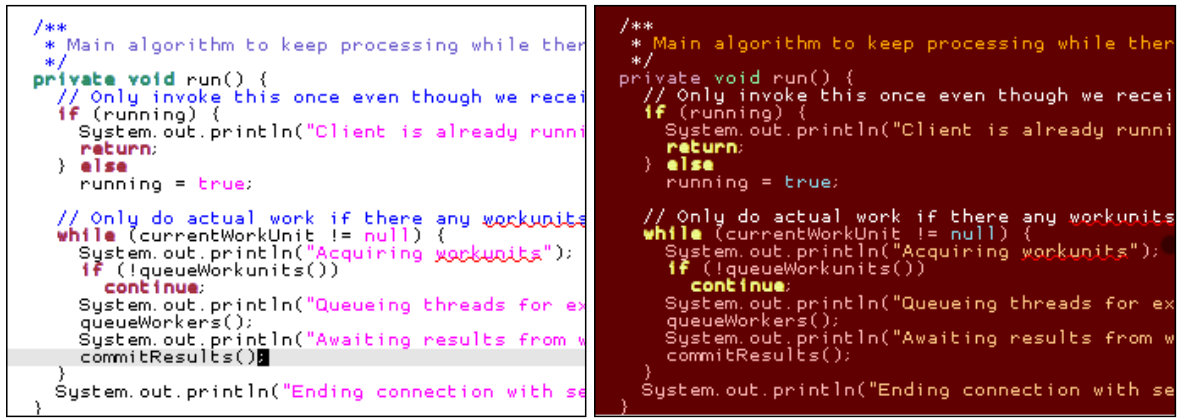
\includegraphics[scale=0.4]{./images/page22.png}
\end{center}

\subsection{个性化高亮}
\label{subsec:personal_highlighting}
在 Vim 中, 与高亮相关的最关键的技术是 \newterm{匹配} (\newterm{matching}).

通过匹配, Vim 几乎可以标记字母, 单词, 数值, 语句, 和文本行的任意一种组合.
你甚至可以决定如何标记它们 (例如 用红色标记错误, 用绿色标记重点内容).

匹配通过下面这个命令完成:
\begin{vimcode}
:match Group /pattern/
\end{vimcode}
命令带有两个参数, 第一个参数是高亮文本时使用的色彩组的名字.
\begin{warning}
    配色方案影响的是全部的颜色设置, 而色彩组只是背景色 (或前景色) 的一个比
    较小的组合, 用户可以将其应用到某个方面, 比如匹配. 当 Vim 启动时, 根据
    所选择的配色方案, 大量的色彩组被设置成某个默认值.

    为了查看所有的色彩组, 执行 \texttt{:so \$VIMRUNTIME/syntax/hitest.vim}.
\end{warning}
\marginpar{23}
第 2 个参数是待匹配的模式. 模式是一个正则表达式, 可以很简单, 也可以极其
复杂 --- 取决于用户想要匹配什么样的内容. 匹配命令的一个比较简单的例子是:
\begin{vimcode}
:match ErrorMsg /^Error/
\end{vimcode}
\begin{center}
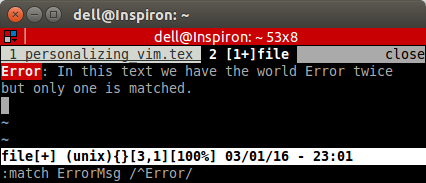
\includegraphics[scale=0.7]{./images/page23.png}
\end{center}

这个命令查找位于行的开始位置的单词 \newterm{Error} (带有脱字符 \texttt{\^}),
如果找到了一个匹配, 就把匹配的文本用色彩组 \texttt{ErrorMsg} 的颜色
标记起来 (通常是红底白字).

如果读者不太喜欢已有的色彩组, 也可以自己定义一个, 定义色彩组的命令是:
\begin{vimcode}
:highlight MyGroup ctermbg=red guibg=red gctermfg=yellow
        guifg=yellow term=bold
\end{vimcode}
这个命令创建了一个名为 \file{MyGroup} 的色彩组, 红底黄字, 在控制台 (Vim)
和 GUI (Gvim) 环境下都是如此. 用户可以根据自己的喜好, 修改下列选项:

\begin{center}
\begin{tabular}{ll}
    \hline
    \texttt{ctermbg}    & 控制台环境下的背景色 \\
    \texttt{guibg}      & Gvim 环境下的背景色 \\
    \texttt{ctermfg}     & 控制台环境下的文本颜色 \\
    \texttt{guifg}      & Gvim 环境下的文本颜色 \\
    \texttt{gui}        & Gvim 环境下的字体格式 \\
    \texttt{term}       & 控制台环境下的字体格式 (比如粗体: bold) \\
    \hline
\end{tabular}
\end{center}

如果使用了已有的色彩组的名字, 那么在接下来的会话中如果用到了该色彩组,
所使用的将会是修改后的效果.

使用匹配命令时, 给定的模式会一直匹配下去, 直到执行一个新的匹配, 或者执行
下列命令:
\begin{vimcode}
:match NONE
\end{vimcode}
\marginpar{24}
匹配命令一次只能匹配一个模式, 但是 Vim 另外提供了 2 个命令用于一次匹配至
多 3 个模式. 命令很容易记忆:
\begin{vimcode}
:2match
:3match
\end{vimcode}
读者也许想知道这些匹配命令应该在什么样的情况下使用, 因为在平时的话这些命令
没什么大用处. 这里有一些例子, 它们展示出了匹配的强大之处.

\subsubsection{示例 1: 用彩色标记某列后面的文字}
\label{subsubsec:mark_color_characters_after_a_certain}
在写邮件时, 一条比较常见的规则是一行的长度不能超过 74 个字符 (在某些古老
的编程语言中, 同样存在这样的规则). 在这种情况下, 当你在一行内写出的字符
数超过某个上限时, 如果 Vim 能够发出提醒那就再好不过了.

只需要下面这个命令就可以完成上面提到的功能:
\begin{vimcode}
:match ErrorMsg /\%>73v.\+/
\end{vimcode}
执行该命令后, 一行内的第 73 个字符之后的那些字符都会被标记成错误. 匹配命令
中含有一个正则表达式, 这个表达式可以拆成:
\begin{center}
\begin{tabular}{ll}
    \hline
    \verb'\%>'  & 匹配该列之后的内容, 列号紧跟在尖括号的右边 \\
    \verb'73'   & 列号  \\
    \verb'v'    & 只能工作在可见的列上面 \\
    \verb'.\+'  & 匹配一个或多个任意的字符 \\
    \hline
\end{tabular}
\end{center}
\begin{center}
    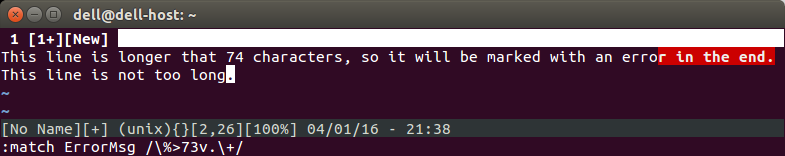
\includegraphics[scale=0.6]{./images/page24.png}
\end{center}
\marginpar{25}
\subsubsection{示例 2: 标记代码中未被用作缩进的制表符}
\label{subsubsec:mark_tabs_not_used_for_indentation_in_code}
编码时, 一条很重要的规则是制表符只被用作缩进代码, 其他地方则不允许使用制表
符. 然而, 对某些人来说常常会忘记该规则. 现在, 只需要一条简单的匹配命令, 就
可以时刻提醒着程序员.

下面这条命令把所有的, 不在行的开始位置上的制表符用错误信息的颜色标记出来:
\begin{vimcode}
:match errorMsg /[^\t]\zs\t\+/
\end{vimcode}
执行完该命令后, 你就可以看到是否违反了规则 --- 把制表符用在了代码内部. 把
命令分解开来看, 它由下列这几个部分组成:
\begin{center}
    \begin{tabular}{ll}
        \hline
        \verb'[^'   & 字符组的开始标记, 组中的字符将不会被匹配到 \\
        \verb'\t'   & 制表符 \\
        \verb']'    & 字符组的结束标记 \\
        \verb'\zs'  & 一个宽度为 0 的匹配, 它把 ``匹配'' 置于一行的开始,
        并忽略任意的空格 \\
        \verb'\t\+' & 匹配一个或多个制表符 \\
        \hline
    \end{tabular}
\end{center}

\begin{center}
    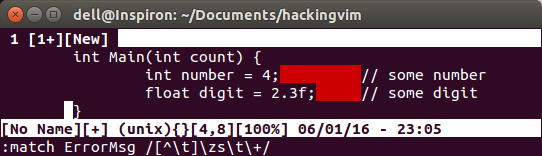
\includegraphics[scale=0.8]{./images/page25.png}
\end{center}

这个命令的意思是: 匹配所有的, 不在行的开始位置上的制表符 (忽略任意的空格).

如果你想用空格来缩进代码, 而不是制表符, 为了检查代码, 只需要把命令改成:
\begin{vimcode}
:match errorMsg /[\t]/
\end{vimcode}
这条命令的意思是: 匹配所有的制表符.
\marginpar{26}
\subsubsection{示例 3: 检查IP地址的有效性}
\label{subsubsec:preventing_errors_caused_by_ip_addresses}

如果用户需要在文本中写上大量的 IP 地址, 难免会出现错误 (例如
123.123.123.256). 为了防止出现这种情况, 可以把以下命令添加到文件
\file{vimrc} 中:
\begin{vimcode}
match errorMsg /\(2[5][6-9]\|2[6-9][0-9]\|[3-9][0-9][0-9]\)[.]
               \[0-9]\{1,3\}[.][0-9]\{1,3\}[.][0-9]\{1,3\}\|
               \[0-9]\{1,3\}[.]\(2[5][6-9]\|2[6-9][0-9]\|\
                \\ \[3-9][0-9][0-9]\)[.][0-9]\{1,3\}[.][0-9]
                \\{1,3\}\|\[0-9]\{1,3\}[.][0-9]\{1,3\}[.]\(2[5]
                \\ \[6-9]\|\2[6-9][0-9]|[3-9][0-9][0-9]\)[.][0-9]\{1,3\}
             \\|[0-9]\{1,3\}[.][0-9]\{1,3\}[.][0-9]\{1,3\}[.]
             \\(2[5][6-9]\|2[6-9][0-9]\|\[3-9][0-9][0-9]\)/

\end{vimcode}
相对于问题来说, 解决方法似乎有点太复杂了, 但请记住, 即使这条命令只能帮助你
一次, 但也值得把它加到配置文件.
\begin{warning}
从另一方面来看, 如果想匹配有效的 IP 地址, 只需要执行:
\begin{vimcode}
    match todo /\(\(25[0-5]\|2[0-4][0-9]\|[01]\?[0-9]
                    [0-9]\?\)\.\)
                    \\ \{3\}\(25[0-5]\|2[0-4][0-9]\|[01]\?
                    [0-9][0-9]\?\)/
\end{vimcode}
\end{warning}

\section{更丰富的状态行}
\label{sec:a_more_informative_status_line}
在 Vim 窗口的底部, 你会发现两样东西:
\begin{itemize}
    \item 命令行缓冲区 (输入命令的地方)
    \item 状态行
\end{itemize}
在默认的配置中, Vim 的状态行非常简单, 信息量也比较少. 状态行的右边显示
的是光标当前所在位置的行号与列号, 左边则是当前打开着的文件名 (如果有的话).

当执行 Vim 命令时, 状态行就会消失, 取而代之的是命令行缓冲区. 如果所执行的
命令带有输出信息, 那么这些信息就会出现在状态行的右侧.
\marginpar{27}
对于简单的文本编辑来说, 这样的状态行已经足够用了. 但是, 如果用户需要天天使用
Vim 来处理不同格式的文件, 那么一条信息量丰富的状态行将会提供很大的帮助.

在这一节, 我们将会通过几个例子, 来说明如何利用简单的办法来配置状态行, 使它
具有更丰富的信息.

配置状态行的命令具有形式:
\begin{vimcmdform}
\texttt{:set statusline}\ \ \textit{format}
\end{vimcmdform}
命令中的 \textit{format} 表示一个格式字符串 (就像 C 程序的 \texttt{printf}),
它描述了状态行的显示格式.

键入 \texttt{:help 'statusline'}, 打开 Vim 的帮助系统, 读者将会看到状态行
可以包含相当多的信息, 其中有些信息在日常工作中非常有用.

作者的状态行信息包括:
\begin{itemize}
    \item 正在编辑的文件名
    \item 正在编辑的文件的格式 (比如 Dos, Unix)
    \item 文件类型
    \item 光标所在位置的字符的 ASCII 码值与十六进制值
    \item 光标所在的行号与列号
    \item 文件的长度 (以行为单位)
\end{itemize}
下面的命令可以让你的 Vim 状态行包含上面提到的所有信息:
\begin{vimcode}
:set statusline=%F%m%r%h%w\ [FORMAT=%{&ff}]\ [TYPE=%Y]\ [ASCII=\%03.3b]\
 [HEX=\%02.2B]\ [POS=%04l,%04v]\ [%p%%]\ [LEN=%L]
\end{vimcode}
我在每一种信息的左右两边都加上了中括号, 这样做就更容易区分彼此. 加中括号只是为
了增加一些视觉效果, 如果不喜欢的话可以直接删掉.

\begin{center}
    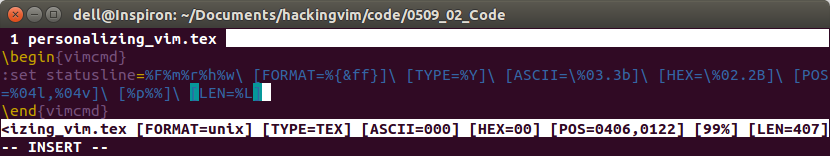
\includegraphics[scale=0.55]{images/page27.png}
\end{center}
\marginpar{28}
然而, 如果在安装 Vim 后没有做过多的配置, 即使执行了上面的状态行命令, 我
们也看不到状态行有什么变化. 这是因为默认情况下 Vim 根本就不会显示状态行,
它只会显示命令行缓冲区及其一小部分信息. 为了让 Vim 显示出真正的状态行, 用户
必须把下面这条命令添加到 \file{vimrc} 文件中. 这条命令确保状态行始终显示在
倒数第 2 行的位置上:
\begin{vimcode}
:set laststatus=2
\end{vimcode}
执行完该命令后, 你就会发现命令行缓冲区有了自己的位置: 窗口的最后一行. 通过
这条命令就可以保证状态行始终拥有自己的显示位置, 而用户也就能一直看到文件的
相关信息. 当然, 状态行会占据编辑区的一部分空间, 但是是否显示状态行由用户来
决定. 下面这条命令关闭状态行, 直到当前会话结束:
\begin{vimcode}
:set laststatus=0
\end{vimcode}

\section{切换菜单与工具条}
\label{sec:toggle_menu_and_toolbar}
如果用户是在控制台中使用 Vim, 就会逐渐习惯没有菜单与工具条的窗口. 但是如果用
的是 Gvim, 你就会发现窗口界面提供了菜单与工具条.

许多人认为应该把额外的空间分配给更重要的文本使用, 而不是菜单与工具条. 如果你
也是这么认为的, 那么你可能希望在使用 Gvim 时, 移除菜单与工具条. 然而, 某
些脚本在菜单中增加许多有用的功能, 而这些功能也只能通过菜单来使用. 解决办法是
根据实际需要, 随时切换菜单与工具条.

下面的代码把组合键 \key{Ctrl+F2} 映射到菜单与工具条的切换操作上, 当然编辑
器用的是 Gvim. 如果喜欢这个功能的话, 可以把代码写到 \file{vimrc} 中.
\begin{vimcode}
map <silent> <C-F2> :if &guioptions =~# 'T' <Bar>
                         \set guioptions-=T <Bar>
                         \set guioptions-=m <bar>
                    \else <Bar>
                         \set guioptions+=T <Bar>
                         \set guioptions+=m <Bar>
                      \endif<CR>
\end{vimcode}
现在, 无论何时, 只要你想关闭菜单与工具条, 好把空间留给文本, 只需要按下
\key{Ctrl+F2} 即可, 如果想它们了, 再按一下 \key{Ctrl+F2}, 它们就回来了.
\marginpar{29}
如果用户希望一直隐藏菜单或工具条, 只需要在 \file{vimrc} 中添加下面两个命令
中的一个即可.

为了完全移除菜单, 添加:
\begin{vimcode}
:set guioptions-=m
\end{vimcode}

为了完全移除工具条, 添加:
\begin{vimcode}
:set guioptions-=T
\end{vimcode}

\begin{warning}
    GUI 的其他设置可以通过命令 \texttt{set guioptions} 完成, 更多的信息可以
    参考\texttt{:help 'guioptions'}.
\end{warning}

\section{添加自己菜单与工具条按钮}
\label{sec:adding_your_own_menu_and_toolbar_buttons}
如果使用的是 Gvim, 那么用户可以把经常用到的功能加入到菜单中. 也许用户并不总
是需要通过菜单来使用某项功能, 但是如果忘记了具体的操作步骤, 我们还可以通过
菜单来完成. 如果用户确实需要快速地执行某个功能, 还可以把它直接加入到 Gvim
的工具条中.

在这一节, 我们将会讨论如何在 Gvim 中制作菜单, 以及如何往工具条中加入额外
的按钮. 先从构造菜单开始.

\subsubsection{添加菜单}
\label{subsubsec:adding_a_menu}
简单来说, 为了构造一个菜单, 只需要为菜单中的每一个菜单项执行对应的命令即可.
只要遵循良好的命名规则, 用户就可以得到一个使用方便, 功能齐全的菜单.
\marginpar{30}
让我们从一个小例子开始, 假设用户想新增一个菜单, 比如缓冲区菜单.

\begin{center}
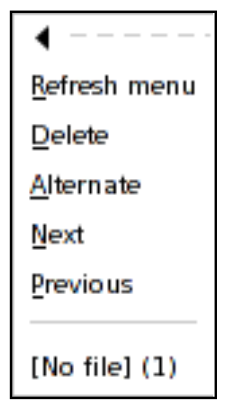
\includegraphics[scale=0.42]{./images/page30.png}
\end{center}

需要用到的命令是:
\begin{vimcmdform}
\texttt{:menu}\ \ \textit{menupath}\ \ \textit{command}
\end{vimcmdform}
这个命令的工作方式类似于命令 \texttt{map}, 后者把命令映射到一个组合键, 而前
者是把命令映射到一个菜单项.

命令带有两个参数. 第 1 个参数是菜单项在菜单中的实际路径, 第 2 个参数是菜单项
被点击时所执行的命令. 举个例子, 假设用户想要在菜单项 \newterm{Tabs} 中, 添加
一个新菜单项 \newterm{Next}, 只需要执行:
\begin{vimcode}
:menu Tabs.Next <ESC>:tabnext<cr>
\end{vimcode}
之后, 你就有了一个新菜单项 \newterm{Tabs}, 它只有一个子菜单项 \newterm{Next}.
现在, 如果用户点击菜单项 \newterm{Next}, 就会执行:
\begin{vimcode}
:tabnext
\end{vimcode}
命令前面的 \texttt{<ESC>} 为的是让 Vim 切换到普通模式,
后面的 \texttt{<cr>} 是真正执行命令的地方. 如果漏掉了 \texttt{<ESC>}, 那么
命令就无法正常地工作. 另外一种办法是根据当前的模式, 在命令前添加特定
的菜单项, 为此, Vim 提供了几个 \texttt{:menu} 的替代命令:
\begin{itemize}
    \item \texttt{:nmenu} 用于 \newterm{普通}(\newterm{Normal}) 模式
    \item \texttt{:imenu} 用于 \newterm{插入}(\newterm{Insert}) 模式, 前置
        \verb'^O'
    \item \texttt{:vmenu} 用于 \newterm{可视}(\newterm{Visual}) 模式, 前置
        \verb'^C', 后置 \verb'^\^G'
    \item \texttt{:cmenu} 用于 \newterm{命令行}(\newterm{Command-line}) 模式,
        前置 \verb'^C', 后置 \verb'^\^G'
    \item \texttt{:omenu} 用于 \newterm{操作挂起} (\newterm{OP-pending})
        模式, 前置 \verb'^C', 后置 \verb'^\^G'
\end{itemize}
\marginpar{31}
前置部分 (\verb'^O' 与 \verb'^C') 用于将 Vim 切换到普通模式.

\verb'^O' (\key{Ctrl+O}) 专门用于插入模式, 因为它会在执行完命令之后让编辑器
重新回到插入模式.

\verb'^\^G' (\key{Ctrl+\textbackslash}, \key{Ctrl+G}) 用于这样一种特殊情况:
全局插入模式被设置为真, 并且 Vim 把插入模式作为默认模式 (此时 Vim
是无模式的), 此时, 它们就可以把模式还原成原来的样子.
\begin{warning}
没必要为每一种模式创建一个同样的菜单项, 这时候只需要使用下面这个命令即可:
\begin{vimcmdform}
\texttt{:amenu}\ \ \textit{menu-path}\ \ \textit{command}
\end{vimcmdform}
这个命令可以根据当前的模式, 设置正确的前置命令与后置命令.
\end{warning}

现在开始创建我们的新菜单 \newterm{Tabs}, 并添加几个新菜单项与功能. 执行了
下面这些命令后, 新菜单就有点像 \newterm{Buffers} 菜单了:
\begin{vimcode}
:amenu Tabs.&Delete :confirm tabclose<cr>
:amenu Tabs.&Alternate :confirm tabn #<cr>
:amenu <silent> Tabs.&Next :tabnext<cr>
:amenu <silent>Tabs.&Previous :tabprevious<cr>
\end{vimcode}
细心的读者会发现这些命令之中又多了点新东西.

第一个是 \texttt{<silent>}, 它可以阻止命令执行过程中, 命令的内容被回显到命令行
缓冲区. 当然, 这个功能只是装饰性的, 相比之下, 菜单路径中的 \verb'&' 就实
用多了. 把字符 \verb'&' 加在菜单路径的最后一个部分的某个字母之前, 就可以为该
菜单项定义一个快捷键. 有了快捷键, 定位并执行菜单项就方便多了.
\begin{center}
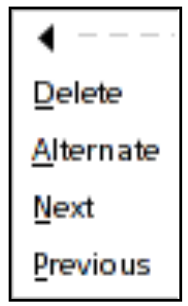
\includegraphics[scale=0.42]{./images/page31.png}
\end{center}
\marginpar{32}
假设用户想通过执行菜单项 \newterm{Tabs | Next} 来切换到下一个标签页, 现在,
只需要按下 \key{Alt + T + N} 即可. \key{Alt + T} 打开 \newterm{Tabs}, 再
按 \key{N} (之所以是 \key{N}, 是因为 \verb'&' 放在 \texttt{Next} 的
\texttt{N} 的前面) 来执行 \newterm{Next}. 如果有其他的菜单项使用了相同的
快捷键字母, 只需要一直按 \key{Alt} 就可以遍历所有的菜单项.
\begin{warning}
    如果用户希望下拉菜单的各项之间用一条横线分开, 可以使用 \texttt{SEP}
    (针对菜单项) 或 ``\texttt{:}'' (针对命令):
\begin{vimcode}
:amenu Tabs.-SEP-:
\end{vimcode}
用户创建的菜单仅对当前会话有效, 如果想要让菜单在下一次启动 Vim 时仍然存在,
可以把菜单的创建命令写到 \file{vimrc} 中 (写到 \file{vimrc} 的命令不需要前
面的冒号 \texttt{:}).
\end{warning}
现在我们已经有了一个简单的 \newterm{Tabs} 菜单, 看起来有点像菜单
\newterm{Buffers}. 不过它还不具备 \newterm{Buffers} 菜单所拥有的列出活动
缓冲区的功能. 缓冲区可以对用户隐藏起来, 而标签页肯定是可见的, 如果读者知道
这点, 就会明白这个功能对标签页来说没什么用处. 换句话说, 用户看见的标签页
就是当前编辑器中所有的标签页, 而且它们的名字都显示在标签的标题栏中.

一个 \newterm{Personal} 菜单可以用来完成许多有趣的事情. 如果用户需要处理多种
类型的文件, 甚至可以启动时为某个特定的文件类型创建菜单, 或者是在同一个菜单
下, 为不同的文件类型搭配不同的子菜单.

只需要遵循菜单路径的命名规范就可以创建出子菜单. 于是, 如果用户想要的菜单是
\newterm{Tabs | Navigation | Next}, 只需要用菜单路径
\texttt{Tabs.Navigation.\&Next} 来添加子菜单项 \newterm{Next}.

\subsubsection{添加工具条图标}
\label{subsubsec:adding_toolbar_icons}

既然我们已经知道了如何创建菜单, 那么给工具条添加自定义的图标就容易多了.
事实上, Vim 把工具条看作是带有特殊名字的菜单. 因此, 给工具条添加图标就像是
给菜单添加菜单项.

对于工具菜单, 为了给它添加一个子项目, 需要使用以 \texttt{ToolBar} 开始的
菜单路径. 为了给工具条添加一个用于执行命令 \texttt{:buffers} (列出打开的
缓冲区) 的子项目, 用户需要执行命令:
\begin{vimcode}
:amenu icon=/path/to/icon/myicon.png ToolBar.Bufferlist :buffers<cr>
\end{vimcode}
\marginpar{33}
当然, 用户必须把图标文件放在某个目录中, 并在命令中给出这个目录.

图标文件的存放目录通过参数 \texttt{icon} 传递给命令 \texttt{amenu}. 如果只
给出了文件名, 而没有给出路径, 那么 Vim 就会在运行时路径的 \texttt{bitmaps/}
目录下搜索图标文件 (运行时路径可以通过 \texttt{:echo \$VIMRUNTIME}
命令获取). 受支持的图标类型依赖于系统.

到现在为止就大功告成了! 执行完命令之后, 用户就可以看到他的图标出现在了工具
条中, 而且处在已有图标的最靠右的位置上. 如果点击该图标, Vim 就会执行命令
\texttt{:buffers}, 显示缓冲区列表.

和菜单一样, 可以通过特定于模式的菜单命令 \texttt{imenu}, \texttt{vmenu},
\texttt{cmenu} 等, 使得工具按钮只会在特定的模式下才会显示出来.

\begin{warning}
默认情况下, 新增的菜单或按钮图标处在已有的菜单或图标的右边, 可以通过优
先级来改变默认行为. 更多的信息请参考 \texttt{help menu-priority} 与
\texttt{:help sub-menu-priority}.
\end{warning}

\section{修改标签页}
\label{sec:modifying_tabs}
Vim 从 7.0 开始支持标签页. 标签页与其他应用程序中的标签不太一样 --- 在
Vim 中, 它是组织打开文件的一种方式. 每一个标签都可以包含若干个缓冲区,
甚至多个窗口.

有了标签页之后, 原来的针对所有缓冲区或窗口的命令 (例如 \texttt{:bufdo},
\texttt{:windo} 和 \texttt{:ball}) 将仅限于当前标签的窗口或缓冲区.

一般情况下, 所有的标签页以一种标签列表的形式呈现在窗口的上方 (就在编辑区
之上). 每一个标签页都有一个标签, 默认是处于当前活动缓冲区的文件名. 如果
一个标签页中同时打开了多个窗口, 那么标签也会显示窗口的数量.
\begin{center}
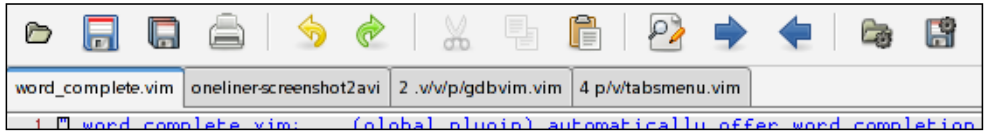
\includegraphics[scale=0.48]{./images/page33.png}
\end{center}
\marginpar{34}
有时候用户希望标签页的标签能提供更多的信息, 比如, 如果用户需要为每一个
项目建一个标签页, 要是能根据项目的名称来对标签页进行命名的话, 那就方便
多了.
\begin{center}

\includegraphics[scale=0.48]{./images/page34-1.png}
\end{center}
设置标签名的方法与状态行 (见 \ref{sec:a_more_informative_status_line} 节)
非常类似. 但是在这里设置的是 \texttt{tabline} 的属性, 而不是
\texttt{statusline}:
\begin{vimcmdform}
\texttt{:set tabline}\ \ \textit{tabline-layout}
\end{vimcmdform}
\begin{center}
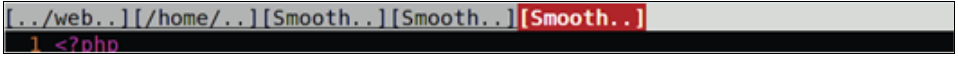
\includegraphics[scale=0.48]{./images/page34-2.png}
\end{center}
如果是 Gvim, 则是
\begin{vimcode}
:set guitablabel
\end{vimcode}

虽然 \texttt{tabline} 的设置方法类似于 \texttt{statusline}, 但是前者会
更麻烦一点. 麻烦的主要原因在于用户必须时刻注意标签页是否处于活跃状态.
我们从 Vim 的一个小例子开始.

如果标签页过多, 标签就会占据太多的空间, 尤其是当它们包含了当前活跃缓冲区
的完整文件名时. 我们希望只显示活跃缓冲区文件名的前 6 个字母, 而且当前
活跃的标签名以红底白字的方式呈现, 就像错误信息那样.

下面的 Vim 脚本程序完成的正是这个功能 (关于如何编写 Vim 脚本程序见第
\ref{chap:basic_vim_scripting} 章).
\begin{vimcode}
function ShortTabLine()
 let ret = ''
 for i in range(tabpagenr('$'))
   " select the color group for highlighting active tab
     if i + 1 == tabpagenr()
     let ret .= '%#errorMsg#'
   else
     let ret .= '%#TabLine#'
    endif

    " find the buffername for the tablabel
       let buflist = tabpagebuflist(i+1)
       let winnr = tabpagewinnr(i+1)
       let buffername = bufname(buflist[winnr - 1])
       let filename = fnamemodify(buffername,':t')
    " check if there is no name
\end{vimcode}
\marginpar{35}
\begin{vimcode}
    if filename == ''
      let filename = 'noname'
    endif
    " only show the first 6 letters of the name  and
    " .. if the filename is more than 8 letters long
    if strlen(filename) >=8
        let ret .= '['. filename[0:5].'..]'
    else
         let ret .= '['.filename.']'
    endif
 endfor

 " after the last tab fill with TabLineFill and reset tab page #
  let ret .= '%#TabLineFill#%T'
  return ret
endfunction
\end{vimcode}

现在, 我们需要把函数添加到 \file{vimrc}, 除此之外, 还要增加一行设置
\texttt{tabline} 的命令, 具体的设置命令是:
\begin{vimcode}
:set tabline=%!ShortTabLine()
\end{vimcode}
命令的执行结果是产生了一个更加紧凑的标签列表, 下面是效果截图:
\begin{center}
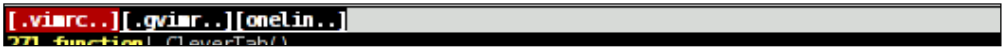
\includegraphics[scale=0.45]{./images/page35.png}
\end{center}

在 Gvim 中设置 \texttt{tabline} 的方法稍有不同, 不过基本思想是一样的. 然而
在 GUI 中, 用户不必考虑活跃标签的颜色, 也不必担心某个标签当前是否处于活跃
状态 --- 这些都是 GUI 自己需要考虑的东西.

于是, 我们可以对函数 \texttt{ShortTabLine()} 进行简化 --- 只需要设置标签
名即可:
\begin{vimcode}
function ShortTabLabel()
 let bufnrlist = tabpagebuflist(v:lnum)
 " show only the first 6 letters of the name + ..
 let label = bufname(bufnrlist[tabpagewinnr(v:lnum) - 1])
 let filename = fnamemodify(label,':h')
 " only add .. if string is more than 8 letters
  if strlen(filename) >=8
     let ret=filename[0:5].'..'
  else
    let ret = filename
 endif
     return ret
 endfunction
\end{vimcode}
\marginpar{36}
我们只要把 \texttt{guitablabel} 的属性设置成函数的输出即可:
\begin{vimcode}
:set guitablabel=%{ShortTabLabel()}
\end{vimcode}
命令的执行效果如下图所示:
\begin{center}
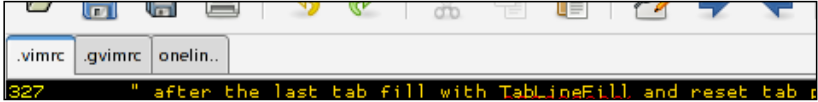
\includegraphics[scale=0.5]{./images/page36}
\end{center}

\begin{warning}
如果用户想要完全移除 Gvim 的标签栏, 只需要执行 \texttt{:set showtabline=0}
(把 \texttt{showtabline} 设置成 1 则会重新显示标签栏).
\end{warning}

现在, 我们已经拥有了只含有有限的信息的标签, 但是我们还是希望能从其他地方
得到信息, 为了完成这个功能需要用到一个小技巧 --- 使用工具提示.

工具提示的优点是当用户没有激活它们时 (例如, 把鼠标移动到标签页的位置上,
就有可能激活标签页的提示信息),
就不会看到这些提示信息. 使用这种方法就可以做到在不填满整个编辑器的情况下,
仍然可以获取到信息.

为了给一个标签页设置工具提示, 需要使用下面的命令:
\begin{vimcode}
:set guitabtooltip
\end{vimcode}
用户需要把它设置成当鼠标经过标签名时, 希望显示出来的信息.

为了测试, 可以先输入一条简单的提示信息:
\begin{vimcode}
:set guitabtooltip='my tooltip'
\end{vimcode}
现在, 工具提示中就可以显示一条静态消息, 但我们需要更多的信息. 我们已经把
文件的路径部分从标签中移走, 但是有时候仍然需要这个信息. 有了工具提示, 我们
就可以把路径信息显示在工具提示中:
\begin{vimcode}
:set guitabtooltip=%!bufname($)
\end{vimcode}

函数可以根据标签的不同, 显示对应的提示信息. 这里, 我们构造了一个小函数, 用
于显示用户会在标签中看到的所有信息, 不过用了一种更加有条理的方式显示出来:
\begin{vimcode}
function! InfoGuiTooltip()
    "get window count
\end{vimcode}
\marginpar{37}
\begin{vimcode}
    let wincount = tabpagewinnr(tabpagenr(),'$')
    let bufferlist=''
   "get name of active buffers in windows
    for i in tabpagebuflist()
        let bufferlist .= '['.fnamemodify(bufname(i),':t').'] '
    endfor
    return bufname($).' windows: '.wincount.' ' .bufferlist ' '
endfunction
\end{vimcode}
然后执行:
\begin{vimcode}
:set guitabtooltip=%!InfoGuiTooltip()
\end{vimcode}
下面这张截图展示了工具提示在 Gvim 中的效果:
\begin{center}
    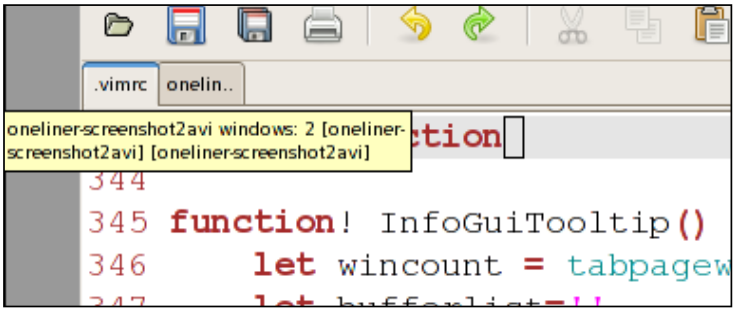
\includegraphics[scale=0.4]{images/page37.png}
\end{center}

用户还可以想到许多其他有趣的用法, 来使用标签与工具提示所提供的功能, 有了前
面的示例, 用户就可以自己动手来实现它们了.

\section{工作区定制}
\label{sec:work_area_personalization}

在这一节, 我们将介绍一些专门针对 Vim 编辑区的设置内容, 之所以介绍这些,
是因为当用户使用 Vim 编辑文本或代码时, 它们可以提高用户的工作效率.

\subsection{为光标添加视觉效果}
\label{subsec:adding_a_more_visual_cursor}
有时候, 用户正在编辑的文件可能带有多种颜色的语法高亮, 这些颜色会干扰用户
追踪光标的位置, 如果可以标记出光标当前所在的行, 那就方便多了.

已经有很多人写过 Vim 脚本来解决这个问题, 但是绝大部分都没什么用 (主要
是因为太慢了, 当文本过长时, 滚动速度就难以接受). 直到 Vim 版本 7, 这个
问题才得以解决, 而且, 它还提供了两种可能的办法来追踪光标的位置.
\marginpar{38}
第一种办法是命令 \texttt{cursorline}, 它可以标记当前光标所在的行, 比如把
当前行的背景色设置成另一种颜色, 而且不会破坏原来的语法高亮. 为了打开它,
执行:
\begin{vimcode}
:set cursorline
\end{vimcode}
命令所使用的颜色由色彩组 \texttt{CursorLine} 定义, 用户可以它设置成任意一种
颜色或风格, 比如:
\begin{vimcode}
:highlight CursorLine guibg=lightblue ctermbg=lightgray
\end{vimcode}
关于色彩组的更多内容请参考 \ref{subsec:personal_highlighting} 节.

\begin{center}
    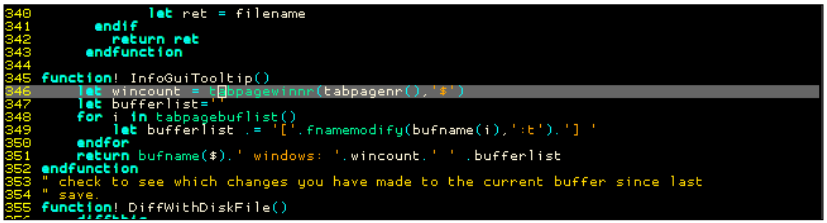
\includegraphics[scale=0.5]{./images/page38-1.png}
\end{center}

如果用户正在编辑的文件含有许多对齐的内容 (比如用制表符分隔的数据), 那么很自然
地就会用到:
\begin{vimcode}
:set cursorcolumn
\end{vimcode}

这个命令标记光标当前所在的列, 例如, 我们可以用另外一种颜色来标记.

和 \texttt{cursorline} 类似, 用户可以修改 \texttt{cursorcolumn} 的标记设置,
它的色彩组是 \texttt{CursorColumn}.

如果同时设置了 \texttt{cursorline} 与 \texttt{cursorcolumn}, 那么光标看起来
就像一对十字线, 这样就再也不用怕把它跟丢了.
\begin{center}
    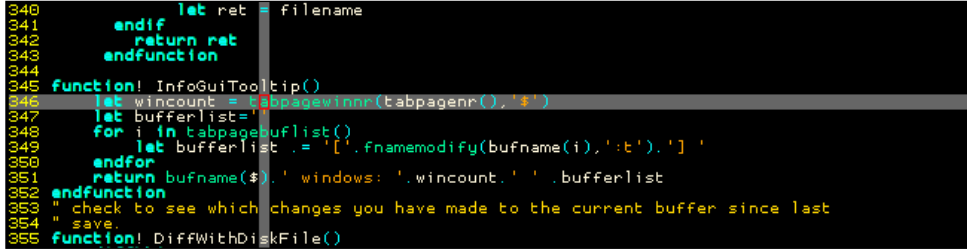
\includegraphics[scale=0.45]{./images/page38-2.png}
\end{center}
\marginpar{39}
\begin{warning}
虽然 \texttt{cursorline} 与 \texttt{cursorcolumn} 是在 Vim 本地实现的, 但是
仍然会影响文件的滚动速度.
\end{warning}

\subsection{添加行号}
\label{subsec:adding_line_numbers}
在编译或调试代码时, 错误信息通常会报告错误所在的行号, 为了定位到这一行, 用户
当然可以从第 1 行开始, 一行一行地往下数, 不过 Vim 提供了更为直接的办法. 只
需要执行 \texttt{:}\textit{XXX} (\textit{XXX} 表示行号), 用户就可以马上到达
第 \textit{XXX} 行.

另一种办法是在普通模式 (按下 \key{Esc} 就可以切换到普通模式) 下, 执行
\textit{XXX}\texttt{gg} 或 \textit{XXX}\texttt{G} (同样, \textit{XXX} 表示
行号). 但是, 如果能随时随地地看到行号可能会更加方便, 这时候就可以执行命令:
\begin{vimcode}
:set number
\end{vimcode}

执行完命令后, 编辑器就会在窗口的左边显示每一行的行号. 默认情况下行号占据 4
个空格的宽度, 3 个用于数字, 1 个用于空格. 这意味着行号所占据的宽度总是一样
的, 除非总行数超过了 999 行. 如果总行数超过了 999 行, 行号所占据的宽度就
会增加一列, 相应地, 文件内容就会右移一列.

当然, 用户可以修改行号占据的列宽, 相应的命令是:
\begin{vimcmdform}
\texttt{:set numberwidth=}\textit{XXX}
\end{vimcmdform}
把 \textit{XXX} 替换成你想要的列宽度.

\begin{warning}
    用户可能希望通过加大列宽度的值, 使得代码与行号之间的间距更大一些,
    但是这个配置无法通过 \texttt{numberwidth} 实现, 因为行号是右对齐的.
\end{warning}
\marginpar{40}

在下面的图片中, 读者可以看到: 当 \texttt{numberwidth} 的值增大时, 行号是如何
右对齐的.

\begin{center}
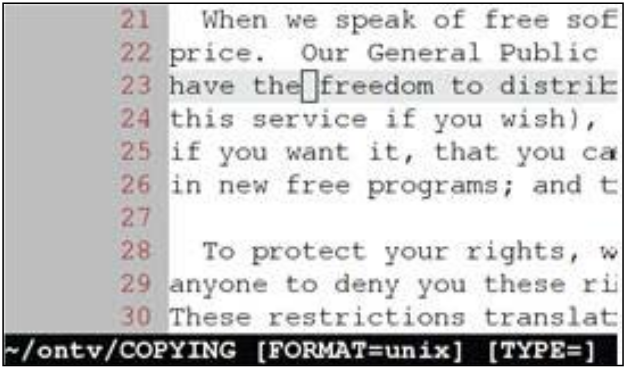
\includegraphics[scale=0.4]{./images/page40.png}
\end{center}

\begin{warning}
    用户可以通过修改色彩组 \texttt{LineNr} 来改变行号及其所在列的风格.
\end{warning}

\subsection{拼写检查}
\label{subsec:spell_checking_your_language}

这个道理我们都懂! 虽然我们对拼写都很在行, 但总会发生拼写错误或打错字的情况.
过去, 为了进行拼写检查 (文本内容已经写在了 Vim 中), 用户需要使用某种拼写检查
工具, 比如 Aspell 或 Ispell. 如果把拼写检查作为最后一项工作, 那么修改起来会
非常得累人, 除非你想过一会儿就检查一遍.

到了 Vim 版本 7, 这种麻烦的拼写检查方式终于可以结束了. 现在, Vim 内置了一个
拼写检查工具, 它支持的语言超过 50 种.

拼写检查工具会在用户输入单词的时候检查拼写的正确性, 所以如果有错误发生的话,
用户可以马上发现.

打开拼写检查的命令是
\begin{vimcode}
:set spell
\end{vimcode}
命令使用默认的语言 (英语) 打开拼写检查, 如果想要使用其他语言, 只需要把
\texttt{spelllang} 设置成该语言的代号即可. 比如:
\begin{vimcode}
:set spelllang=de
\end{vimcode}
\marginpar{41}
在这个命令中语言被设置为德语. 同一种语言可以用多种形式的格式来表达, 比如美式
英文可以写成:
\begin{itemize}
    \item \texttt{en\_us}
    \item \texttt{us}
    \item \texttt{American}
\end{itemize}

语言的名字甚至可以是专业名词, 比如 \texttt{medical}. 如果 Vim 无法识别用户
输入的语言名字, 那么在执行属性设置命令时, 它就会高亮显示无法识别的语言名字.

\begin{warning}
    如果把 \texttt{spelllang} 设置成某个还没有安装的语言, Vim 就会询问用户
    是否自动从 Vim 主页上下载对应的语言.
\end{warning}

对我个人来说, 我经常要用 Vim 同时处理不同的语言, 而且我并不想每次都告诉 Vim 我
现在用的是什么语言.

对此 Vim 也有解决办法. 只要在设置属性 \texttt{spelllang} 时, 给它同时带上
多种语言即可 (语言之间用逗号分开), 这样 Vim 就可以用多种语言来进行语法检查.
\begin{vimcode}
:set spelllang=en,da,de,it
\end{vimcode}
Vim 将会按照顺序, 轮流根据每一种语言检查单词的拼写是否正确. 如果单词对某一种
语言来说是正确拼写的, 那它就不会被标记错误. 当然, 这就意味着如果有一个
单词的拼写本来是错误的, 可是碰巧它在另一种语言中是正确的, 那么它也不会被
当成错误, 这将会引入一个难以察觉的错误.

\begin{warning}
    用户可以到 Vim 的 FTP 站点 \url{ftp://ftp.vim.org/pub/vim/runtime/spell}
    上找到大量的语言包.
\end{warning}

Vim 与 Gvim 对错误单词的标记方法稍有不同.

在普通的 Vim 中, 拼写错误的单词使用色彩组 \texttt{SpellBad} 标记 (默认情况下
是红底白字).
\marginpar{42}

在 Gvim 中, 拼写错误的单词用红色的波浪线标记, 当然, 这也可以通过设置色彩组
来改变颜色 (关于如何设置色彩组见 \ref{subsec:personal_highlighting} 节).

\begin{center}
    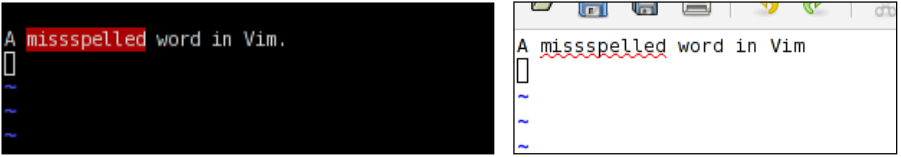
\includegraphics[scale=0.5]{./images/page42-1.png}
\end{center}

无论用户是在什么时候碰到拼写错误的单词, 都可以向 Vim 询问正确的拼写方式.
为此, 需要把光标置于单词中, 并切换到普通模式 (按 \key{Esc}), 然后按
\texttt{z=}.

\begin{center}
    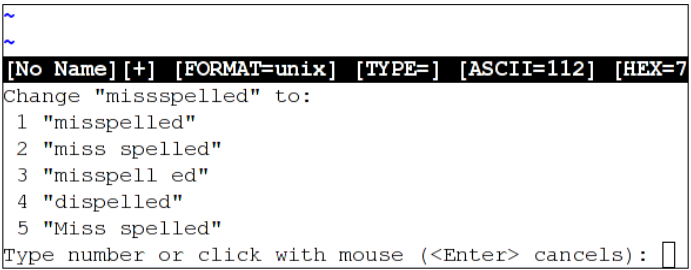
\includegraphics[scale=0.5]{./images/page42-2.png}
\end{center}

如果可能的话, Vim 将会猜测用户试图输入的单词的正确形式, 并给出一个候选列表.
在每个候选单词的前面都有一个数字, 如果其中有你想要的单词, 就输入单词前面的
数字或者单词本身, 然后按 \key{Enter}.

Vim 会给出一长串的候选单词, 除非用户把单词完全拼写错了, 否则的话, 单词的正
确形式应该就在候选单词的前 5 个中, 如果用户不想看到一长串的列表, 那么他就
可以用命令
\begin{vimcmdform}
\texttt{:set spellsuggest=}\textit{X}
\end{vimcmdform}
来限制列表的长度, 其中 \textit{X} 是列表的最大长度.
\marginpar{43}

\subsection{添加帮助性的工具提示}
\label{subsec:adding_helpful_tool_tips}

在 \ref{sec:modifying_tabs} 节, 我们学习了如何利用工具提示, 使得在占据较少
空间的情况下, 存放更多的信息, 以此为基础, 我们将把工具提示应用在编辑器的其中
地方.

编辑区是 Vim 中面积最大的部分, 所以, 为什么不利用工具提示, 在编辑区中添加
一些额外的信息呢?

在 Vim 中, 编辑区的工具提示称为 balloons, 只在当鼠标停在组成这个单词的
某个字符的上方时, 提示信息才会显示出来. 为了使用 balloons, 用户必须知道
下面这几个命令:
\begin{itemize}
    \item 第 1 个命令是在 Vim 中启用 balloons:
    \begin{vimcode}
    :set ballooneval
    \end{vimcode}
    \item 第 2 个命令告诉 Vim 在显示信息之前需要等待多长时间 (默认是 600
    毫秒):
    \begin{vimcode}
    :set balloondelay=400
    \end{vimcode}
    \item 最后一个命令是设置信息的内容:
    \begin{vimcode}
    :set balloonexpr="textstring"
    \end{vimcode}
    信息的内容既可以是静态的文本字符串, 也可以是函数的返回值.
\end{itemize}

为了访问鼠标所在的位置的相关信息, Vim 提供了一些变量:
\begin{center}
\begin{tabular}{ll}
    \hline
    \texttt{v:beval\_bufnr} & 鼠标所在区域的缓冲区个数 \\
    \texttt{v:beval\_winnr} & 鼠标所在区域的窗口的个数 \\
    \texttt{v:beval\_lnum}  & 鼠标所在的行号 \\
    \texttt{v:beval\_col}   & 鼠标所在的列号 \\
    \texttt{v:beval\_text}  & 触发提示信息的字符所在的单词 \\
    \hline
\end{tabular}
\end{center}
\marginpar{44}
有了这些变量之后, 我们来看一些具体的例子.

\subsubsection{示例 1}
\label{subsubsec:example_1}

第 1 个例子基于 Vim 的帮助系统, 它展示了如何编写一个简单的函数, 用来显示
所有的变量.
\begin{vimcode}
function! SimpleBalloon()
   return 'Cursor is at line/column: ' . v:beval_lnum .
		\'/' . v:beval_col .
		\ ' in file ' .  bufname(v:beval_bufnr) .
		\ '. Word under cursor is: "' . v:beval_text . '"'
endfunction
set balloonexpr=SimpleBalloon()
set ballooneval
\end{vimcode}
脚本的运行结果如下图所示:
\begin{center}
    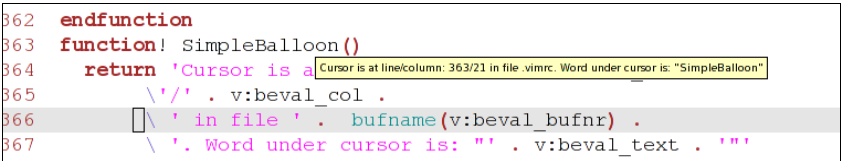
\includegraphics[scale=0.5]{./images/page44.png}
\end{center}

\subsubsection{示例 2}
\label{subsubsec:example_2}

现在来看一个更高级的例子, 这个例子把 balloons 应用到编辑区的特定区域上.
在这个例子中, 我们将会开发一个函数, 这个函数可以同时显示两种 balloons
信息:
\begin{itemize}
    \item 拼写错误的单词: 这个 balloons 信息给出候选单词.
    \item 折叠的文本: 这个 balloons 信息给出被折叠的文本的预览.
\end{itemize}

现在, 我们需要知道什么样的函数可以帮助我们判断鼠标是停在拼写错误的单词上,
还是停在一个折叠行 (这个折叠行代表了折叠后的多个文本行) 上.

为了判断单词的拼写是否错误, 我们需要打开拼写检查功能:
\begin{vimcode}
:set spell
\end{vimcode}
\marginpar{45}
打开后, 如果鼠标所在的单词有拼写错误, 被调用的内置拼写检查函数 ---
\texttt{spellsuggest()} --- 就会返回候选单词. 所以, 为了判断某个单词的拼写
是否有错, 只需要检查 \texttt{spellsuggest()} 的返回值即可. 不过有一点需要
注意, 即使单词没有拼错, \texttt{spellsuggest()} 也可能会返回候选单词.
为了解决这个问题, 在把单词交给 \texttt{spellsuggest()} 之前, 需要用另一个
函数过滤一下, 这个函数叫作 \texttt{spellbadword()}. 它的作用是把光标移动
到句子中第一个拼错的单词上, 然后再返回这个单词. 如果我们输入一个拼写正确
的单词, 那么它应该不返回任何信息. 如果没有单词被输送给
\texttt{spellsuggest()}, 那它就不会返回候选单词, 于是, 我们现在就可以检查
某个单词是否有拼写错误.

检查某个单词是否在一个折叠块中更简单. 以鼠标所在的行号作为输入参数,
调用函数 \texttt{foldclosed()} (回忆变量 \texttt{v:beval\_lnum}), 它会
返回鼠标所在的折叠块的第一行的行号, 如果不是折叠块, 就返回 \texttt{-1}.
换句话说, 如果 \texttt{foldclosed(v:beval\_lnum} 返回除了 \texttt{-1}
之外的其他值, 那么我们就在一个折叠块中.

把上面提到的所有内容都搜集起来, 就得到了下面这个函数:
\begin{vimcode}
function! FoldSpellBalloon()
  let foldStart = foldclosed(v:beval_lnum )
  let foldEnd   = foldclosedend(v:beval_lnum)
  let lines = []
  " Detect if we are in a fold
  if foldStart < 0
    " Detect if we are on a misspelled word
    let lines = spellsuggest( spellbadword(v:beval_text)[ 0 ], 5, 0 )
  else
    " we are in a fold
    let numLines = foldEnd - foldStart + 1
    " if we have too many lines in fold, show only the first 14
    " and the last 14 lines
    if ( numLines > 31 )
      let lines = getline( foldStart, foldStart + 14 )
      let lines += [ '-- Snipped ' . ( numLines - 30 ) . ' lines --' ]
      let lines += getline( foldEnd - 14, foldEnd )
    else
      "less than 30 lines, lets show all of them
      let lines = getline( foldStart, foldEnd )
    endif
  endif
  " return result
\end{vimcode}
\marginpar{46}
\begin{vimcode}
  return join( lines, has( "balloon_multiline" ) ? "\n" : " " )
endfunction

set balloonexpr=FoldSpellBalloon()
set ballooneval
\end{vimcode}

这些帮助性的 balloons 可以极大地提高用户的工作效率, 下面的图展示了折叠块
的预览效果:
\begin{center}
    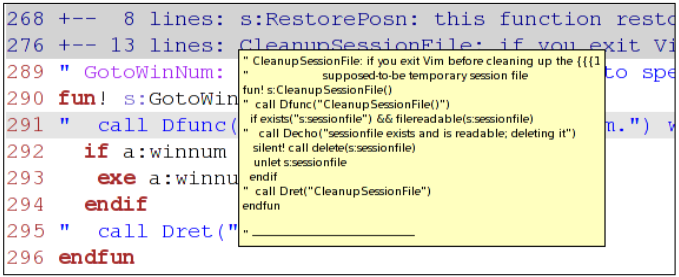
\includegraphics[scale=0.4]{./images/page46-1.png}
\end{center}

如果把它应用到一个拼写错误的单词上, 得到的就是:
\begin{center}
    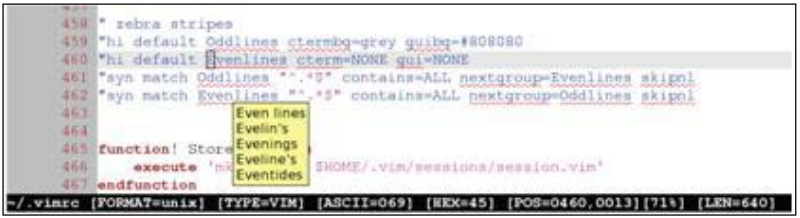
\includegraphics[scale=0.4]{./images/page46-2.png}
\end{center}

\begin{warning}
    在第 \ref{chap:production_boosters} 章, 读者将会学习到如何利用行
    的折叠来提高 Vim 的生产力.
\end{warning}

\subsection{使用缩写}
\label{subsec:using_abbreviations}

对于重复性工作我们都深有体会, 但这种现象却恰恰是 Vim 想要极力避免的.
\marginpar{47}
Vim 的设计哲学是: 如果用户曾经为某件事物写过一次, 那就不需要再写第二次.
然而, 如果用户发现自己正在一次又一次地输入同一个内容, 那就说明他需要找到
一个更好的办法.

为了避免多次输入同一个内容, 用户可以使用 缩写 (abbreviations).

根据不同的使用模式, 可以使用以下三个命令来创建缩写:
\begin{itemize}
    \item \texttt{:abbreviate}: 创建在所有模式中均可使用的缩写
    \item \texttt{:iabbrev}: 创建只能在插入模式中使用的缩写
    \item \texttt{:cabbrev}: 创建只能在命令行中使用的缩写
\end{itemize}

上面所说的三个命令都需要两个参数 --- 文本的缩写形式与完整形式.

现在, 让我们用一个简单的例子来说明在什么情况下应该使用缩写.

\subsubsection{用缩写来快速插入地址}
\label{subsubsec:using_abbreviations_for_quick_address_insertion}
在过去的几年我更换了几次住所, 所以我的一个经常性的工作就是把我的新住址
告诉给别人. 为地址准备一个缩写并不会花上太多时间, 有了缩写之后, 就不用每
次都把整个地址都写出来.

命令的具体形式是:
\begin{vimcode}
:iabbrev myAddr 32 Lincoln Road, Birminham B27 6PA, United Kingdom
\end{vimcode}
每当我想要输入自己的地址时, 我只需要键入 \texttt{myAddr}, 紧接着按一下空格
键, Vim 就会把 \texttt{myAddr} 自动地扩展为完整的地址.

Vim 非常聪明, 它可以判断用户是在输入一个缩写词, 还是仅仅在输入另一个单词
的某个部分, 所以它只会在我输入缩写词并按了空格键之后, 才把缩写扩展为完整
的字符串. 如果在输完缩写词之后, 紧跟着的是一个普通的字母, 那么 Vim 就会知
道用户并不是在输入某个缩写词, 自然也就不会发生扩展. 有关缩写词 \texttt{abc}
的例子如下:
\begin{center}
\begin{tabular}{ll}
    \hline
    \texttt{abc<space>}     & 扩展 \\
    \texttt{abc<enter>}     & 扩展 \\
    \texttt{123abc<space}   & 不会扩展, 因为缩写词现在是某个单词的一部分 \\
    \texttt{abcd<space>}    & 不会扩展, 因为在缩写词后面紧跟着的是字母 \\
    \texttt{abc}            & 不会扩展, 除非接下来输入另一个特殊字符 \\
    \hline
\end{tabular}
\end{center}
\marginpar{48}

为了避免每次都执行一次缩写命令, 用户可以把它们放在 \texttt{VIMHOME} 的某个
文件中, 假设文件名就叫 \texttt{abbreviations.vim}, 然后在文件 \texttt{vimrc}
使用命令 \texttt{source} 来使能该文件 (需确保该文件是可读的):
\begin{vimcode}
:source $VIM/abbreviations.vim
\end{vimcode}

每当用户需要一个新的缩写词时, 可以先在编辑器中创建缩写词, 然后再把它加入到文件
\texttt{abbreviations.vim}.

也许读者已经意识到, 除了这些, 缩写可以应用在其他有趣的地方. 但无论如何,
这里有一些例子, 或许可以向你提供一些思路:
\begin{itemize}
    \item 纠正常见的拼写错误:
\begin{vimcode}
:iabbr teh the
\end{vimcode}
    \item 编程模版
\begin{vimcode}
:iabbr forx for(x=0;x<100;x++){<cr><cr>}
\end{vimcode}
    \item 更短的命令
\begin{vimcode}
:cabbr csn colorscheme night
\end{vimcode}
\end{itemize}

如果读者发现了一个新的缩写, 或许它看起来有点古怪, 刚开始用的时候还有点麻烦,
但是读者应该习惯这一点, 因为到最后将会发现, 它可以帮助你节省大量的时间.
用户唯一所要做的事就是把新的缩写加入到配置文件中, 然后再重新加载即可.

但是有时候缩写可能会比较恼人, 因为它自作聪明地扩展了用户并不希望扩展的单词.
比如, 用户有一个地址的缩写词是 ``addr'', 但是用户其实想写的是单词
``addressed''. 在这种情况下, 缩写功能会突然冒出来, 用户也很难轻易地写出他
所想要的单词.

一种解决办法是在插入单词之前调用一个函数, 该函数询问用户是否使用缩写
扩展功能.

该函数的一种实现是:
\begin{vimcode}
function! s:AbbrAsk(abbr,expansion)
    let answer = confirm("use the abbreviation '" . a:addr . "'?",
        "&Yes\n&No", 1)
    return answer ==  1 ? a:expansion : a:abbr
endfunction
\end{vimcode}
\marginpar{49}

函数需要两个参数, 第 1 个参数是缩写诩, 第 2 个参数缩写词扩展后的形式,
对我们的例子来说, 该函数的用法是:
\begin{vimcode}
:iabbrev <expr> addr <SID>AbbrAsk('addr', "your full address here")
\end{vimcode}

所以, 当用户写下 \texttt{addr} 时, Vim 会询问用户是否对缩写词进行扩展.

\subsection{修改按键绑定}
\label{subsec:modifying_key_bindings}

我们中的大部分人可能除了 Vim 之外, 还用过其他的编辑器, 正因为如此, 我们经常
需要用到一些特定的快捷键来完成不同的任务.

虽然 Vim 中的快捷键绑定在最开始设计时都是力求使用方便且快速, 但是在某些情况
下, 使用用户已经熟悉的快捷键可能会更快.

为了完成这个功能, Vim 几乎可以对任何一个单独的按键进行重新绑定.

在这一节, 我们将会学习到在不同的模式下, 如何对 Vim 的按键绑定进行修改.

处理按键绑定的命令主要有:
\begin{itemize}
    \item \texttt{:map}  用于普通模式, 插入模式, 可视模式, 与命令行模式
    \item \texttt{:imap}  只能用于插入模式
    \item \texttt{:cmap}  只能用于命令行模式
    \item \texttt{:nmap}  只能用于普通模式
    \item \texttt{:vmap}  只能用于可视模式
\end{itemize}

每一个命令都需要两个参数, 第一个参数是被绑定的按键, 第二个参数是被绑定的命
令. 现在让我们看几个例子.

假设用户不太习惯在普通模式下用命令 \texttt{:w} 来保存文件, 因为你已经习惯了
\key{Ctrl-S}, 并且想继续使用下去.
\marginpar{50}
解决这个问题的一个映射可以是:
\begin{vimcode}
:map <C-s> :w<cr>
\end{vimcode}

注意命令中的 \texttt{<C-s>}, 这是组合键 \key{Ctrl+S} 在 Vim 中的表示方式.
除了 \texttt{C} (\key{Ctrl}), 用户还可以用 \texttt{A} (\key{Alt}) 或
\texttt{M} (\key{Meta}). 命令末尾的 \texttt{<cr>} 是真正执行命令的地方.
如果缺了它, 命令只会被显示在命令行中, 而不会被执行.

除了 \texttt{<cr>}, 还有其他的一些用来表示按键的特殊记号, 下面这张表显示了
比较常见的记号:
\begin{center}
    \begin{tabular}{ll}
        \hline
        按键        & 记号  \\
        \hline
        \texttt{<BS>}   & 退格 \\
        \texttt{<Tab>}   &  制表符 \\
        \texttt{<CR>}   & 回车  \\
        \texttt{<Enter>}   & 回车 \\
        \texttt{<Return>}   & 回车 \\
        \texttt{<Esc>}   & 转义 \\
        \texttt{<Space>}   & 空格 \\
        \texttt{<Up>}   & 方向键, 上 \\
        \texttt{<Down>}   & 方向键, 下 \\
        \texttt{<Left>}   & 方向键, 左 \\
        \texttt{<Right>}   & 方向键, 右 \\
        \texttt{<F1>} - \texttt{<F12>}  & 功能键, \texttt{F1} 到
            \texttt{F12} \\
        \texttt{\#1}, \texttt{\#2},...,\texttt{\#9}, \texttt{\#0}  & 功能键, 从
            \texttt{F1} 到 \texttt{F10} \\
        \texttt{<Insert>}   & 插入 \\
        \texttt{<Del>}   & 删除 \\
        \texttt{<Home>}   & 返回到行的开始 \\
        \texttt{<End>}   & 返回到行的结束 \\
        \texttt{<PageUp>}   & 下一页 \\
        \texttt{<PageDown>}   & 上一页 \\
        \hline
    \end{tabular}
\end{center}

如果用户只可能在插入模式下才会保存文件, 而且在保存之后想要继续在插入模式下
工作, 那么用户就需要执行:
\begin{vimcode}
:imap <C-s> <esc>:w<cr>a
\end{vimcode}
\marginpar{51}

之后, \key{Ctrl+S} 就被映射成几个按键的组合. 首先, 按下 \texttt{<esc>}
(\key{Escape} 键), 使 Vim 从插入模式进入到普通模式. 然后, 使用
\texttt{:w<cr>} 完成实际的文件保存操作. 最后, 用 \texttt{a} 再回到插入模式,
并将光标移到行的末尾.

用户可以通过映射来适应大多数应用程序的标准的 复制/粘贴/剪切/保存 快捷键,
具体来说, 可以这样做:
\begin{vimcode}
" save file (ctrl-s)
:map <C-s> :w<cr>
" copy selected text (ctrl-c)
:vmap <C-c> y
" Paste clipboard contents (ctrl-v)
:imap <C-p> <esc>P
" cut selected text (ctrl-x)
:vmap <C-x> x
\end{vimcode}

如果是 Gvim, 甚至可以打开 \texttt{Save-as} 与 \texttt{Open} 的对话框:
\begin{vimcode}
" Open new file dialog (ctrl-n)
:map <C-n> :browse confirm e<cr>
" Open save-as dialog (ctrl-shift-s)
:map <C-S-s> :browse confirm saveas<cr>
\end{vimcode}

用户可能会遇到这样一种情况: 组合键的第一个按键已经绑定到了 Vim 的某个功能
上. 举个例子, 按键 \verb'$', 它的功能是把光标移到一行的末尾. 用户可能希望
为 \verb'$1' 新绑定一个功能, 为 \verb'$2' 绑定另一个功能, 如此等等. 具体的
形式是:
\begin{vimcode}
:map $1 :MyFunction1()<cr>
:map $2 :MyFunction2()<cr>
\end{vimcode}

现在, 如果用户按下了 \key{\$}, Vim 就会等待一秒, 等待另一个按键被按下,
如果在这一秒之内没有按键按下, Vim 就会执行原来的功能: 把光标移到一行的末尾.
相反, 如果在 1 秒之内用户按下了 \key{1}, Vim 就会执行函数
\texttt{MyFunction1()}.

有了按键映射功能, 用户就有了一个强大的工具来根据自己的需要, 对 Vim 进行
修改.

\begin{tips}
    关于映射的更多的帮助信息, 可以查看 Vim 的帮助系统: \texttt{:help
    key-mapping}.
\end{tips}
\marginpar{52}
\section{小结}
\label{sec:personalizing_vim_summary}

在这一章, 我们学习了如何根据自己的具体需求来配置 Vim.

我们首先学习了字体与配色方案的基本修改方法, 通过它们来修改 Vim 的外观.

接下来, 我们讨论了如何使用颜色来标记搜索匹配, 从而使得它们更容易被识别.

为了最大限度地利用 Vim, 用户通常将大部分的区域用于编辑, 而将小部分区域用于
其他功能. 因此, 我们介绍了如何配置状态行与标签列表, 使得它们占用更少的空间,
同时提供更多的信息.

虽然菜单栏与工具栏不是非常重要, 而且还会占用本来就有限的屏幕空间, 但是它们
仍然可以提供很大的用处. 在这一章, 我们学习了如何在菜单栏中添加自定义的菜单,
以及如何在工具栏中添加图标.

为了让编辑区更符合用户的需求, 可以对它进行许多修改. 在这一章, 我们简单地讨
论了编辑区, 叙述了如何获得一个更好, 更具视觉效果的光标, 以及如何在编辑区中显
示行号.

我们还介绍了在 Vim 中如何进行拼写检查, 从而避免拼错单词. 如果拼写检查也无法
纠正错误, 还可以使用缩写.

最后, 我们介绍了按键绑定, 这样用户就可以继续使用其他编辑器的快捷键而养成的
习惯.

现在, 用户已经拥有了一个完全定制化的 Vim, 接下来, 用户可以更加深入地学习
如何在多个文件中更快速地跳转.
